\documentclass[tikz,border=10pt]{standalone}
\usepackage{tikz}
\usetikzlibrary{arrows.meta,positioning,calc}

\begin{document}
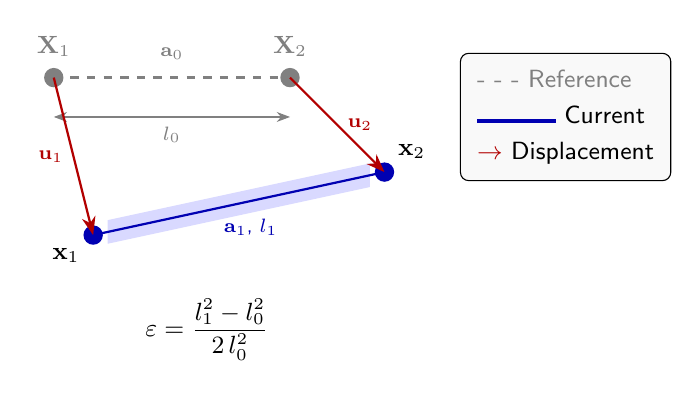
\begin{tikzpicture}[
    node font=\sffamily,
    >=Stealth,
    node dot/.style={circle, fill=black, inner sep=0pt, minimum size=7pt},
    dof arrow/.style={->, thick, color=green!60!black},
]

% === Reference Configuration (dashed) ===
\coordinate (X1) at (0,2);
\coordinate (X2) at (3,2);

\draw[thick, dashed, gray] (X1) -- (X2);
\node[node dot, fill=gray] at (X1) {};
\node[node dot, fill=gray] at (X2) {};

\node[above=4pt, font=\small\itshape, gray] at (X1) {$\mathbf{X}_1$};
\node[above=4pt, font=\small\itshape, gray] at (X2) {$\mathbf{X}_2$};

% Length label
\draw[<->, gray, thin] (0,1.5) -- (3,1.5) node[midway, below, font=\scriptsize] {$l_0$};
\node[font=\scriptsize, gray] at (1.5,2.3) {$\mathbf{a}_0$};

% === Current Configuration (solid) ===
\coordinate (x1) at (0.5,0);
\coordinate (x2) at (4.2,0.8);

% Bar element
\fill[blue!15] ($(x1)!0.05!(x2) + (0,0.15)$) -- ($(x1)!0.05!(x2) + (0,-0.15)$) -- 
               ($(x2)!0.05!(x1) + (0,-0.15)$) -- ($(x2)!0.05!(x1) + (0,0.15)$) -- cycle;
\draw[thick, blue!70!black] (x1) -- (x2);

\node[node dot, fill=blue!70!black] at (x1) {};
\node[node dot, fill=blue!70!black] at (x2) {};

\node[below left=2pt, font=\small\itshape] at (x1) {$\mathbf{x}_1$};
\node[above right=2pt, font=\small\itshape] at (x2) {$\mathbf{x}_2$};

% Length label
\node[font=\scriptsize, blue!70!black] at (2.5,0.1) {$\mathbf{a}_1$, $l_1$};

% Displacement vectors
\draw[->, thick, red!70!black] (X1) -- (x1) node[midway, left, font=\scriptsize] {$\mathbf{u}_1$};
\draw[->, thick, red!70!black] (X2) -- (x2) node[midway, right, font=\scriptsize] {$\mathbf{u}_2$};

% Legend
\node[draw, rounded corners=3pt, fill=gray!5, inner sep=6pt, font=\small, align=left] 
    at (6.5,1.5) {
    \textcolor{gray}{- - - Reference}\\[2pt]
    \textcolor{blue!70!black}{\rule{1cm}{1.5pt}} Current\\[2pt]
    \textcolor{red!70!black}{$\rightarrow$} Displacement
};

% Green-Lagrange strain formula
\node[font=\small, align=center] at (2,-1.2) {
    $\displaystyle \varepsilon = \frac{l_1^2 - l_0^2}{2\,l_0^2}$
};

\end{tikzpicture}
\end{document}
